%%%%%%%%%%%%%%%%%%%%%%%%%%%%%%%%%%%%%%%%%%%%%%%%%%%%%%%%%%%%%%%%%%%%%%
% Overleaf (WriteLaTeX) Example: Molecular Chemistry Presentation
%
% Source: http://www.overleaf.com
%
% In these slides we show how Overleaf can be used with standard 
% chemistry packages to easily create professional presentations.
% 
% Feel free to distribute this example, but please keep the referral
% to overleaf.com
% 
%%%%%%%%%%%%%%%%%%%%%%%%%%%%%%%%%%%%%%%%%%%%%%%%%%%%%%%%%%%%%%%%%%%%%%

\documentclass{beamer}

\mode<presentation>
{
  \usetheme{Madrid}       % or try default, Darmstadt, Warsaw, ...
  \usecolortheme{default} % or try albatross, beaver, crane, ...
  \usefonttheme{default}    % or try default, structurebold, ...
  \setbeamertemplate{navigation symbols}{}
  \setbeamertemplate{caption}[numbered]
} 

\usepackage[english]{babel}
\usepackage[utf8x]{inputenc}
\usepackage{graphicx}
\usepackage{hyperref}
  \hypersetup{colorlinks=true}
  \hypersetup{urlcolor=blue}
  \hypersetup{linkcolor = .}
\usepackage{xcolor}
\usepackage{siunitx}
  \sisetup{separate-uncertainty = true}
\usepackage{physics}
\usepackage[font=small,labelfont=bf,justification=centering]{caption}
\usepackage{subcaption}
\usepackage[en-GB]{datetime2}
\usepackage{overpic}
\usepackage{feynmp}
\DeclareGraphicsRule{*}{mps}{*}{}
\usepackage{scalerel}
\newcommand{\mylbrace}[2]{\vspace{#2pt}\hspace{6pt}\scaleleftright[\dimexpr5pt+#1\dimexpr0.06pt]{\lbrace}{\rule[\dimexpr2pt-#1\dimexpr0.5pt]{-4pt}{#1pt}}{.}}
\newcommand{\myrbrace}[2]{\vspace{#2pt}\scaleleftright[\dimexpr5pt+#1\dimexpr0.06pt]{.}{\rule[\dimexpr2pt-#1\dimexpr0.5pt]{-4pt}{#1pt}}{\rbrace}\hspace{6pt}}
\usepackage{ulem} % Line across text
\newcommand{\white}[1]{{\textcolor{white}{#1}}} % White text

% Here's where the presentation starts, with the info for the title slide
\title[$h^+h^-\pi^+\pi^-$]{Model-independent measurement of $\gamma$ in $B^\pm\to[h^+h^-\pi^+\pi^-]_Dh^\pm$ at LHCb and BESIII}

\author{Martin Tat}
\institute{Oxford LHCb}
\date{22nd April 2024}

\titlegraphic{
\includegraphics[height = 2cm]{lhcb.jpg}\hspace{1cm}~%
              
\includegraphics[height = 2cm]{OxfordLogo.pdf}\hspace{1cm}~%
              
\includegraphics[height = 2cm]{bes3.jpg}}

\begin{document}

\begin{frame}
  \titlepage
\end{frame}

% These three lines create an automatically generated table of contents.
%\begin{frame}{Outline}
%  \tableofcontents
%\end{frame}

\section{Introduction}

\begin{frame}{Introduction}
  \begin{center}
    \large{Last presentation since starting my PhD journey 1295 days ago!}
  \end{center}
  \vspace{0.1cm}
  \begin{enumerate}
    \setlength\itemsep{0.7em}
    \item{October 2020: Sensitivity studies with $B^\pm\to [K^+K^-\pi^+\pi^-]_DK^\pm$}
    \item{April 2021: First data fit reveals large tension in $\gamma$}
  \end{enumerate}
  \begin{figure}
    \centering
    
\includegraphics[width = 0.45\textwidth]{Plots/GammaTensionMeme.jpg}
  \end{figure}
  \begin{enumerate}
    \setlength\itemsep{0.7em}
    \setcounter{enumi}{3}
    \item{January 2023: Model-dependent $\gamma$ publication with $3~\sigma$ tension}
    \item{March 2024: BESIII $c_i$/$s_i$ analysis approved by review committee}
    \item{April 2024: Presented $B^\pm\to [h^+h^-\pi^+\pi^-]_Dh^\pm$ to B2OC}
  \end{enumerate}
\end{frame}

\begin{frame}{Recap of BESIII $D^0\to K^+K^-\pi^+\pi^-$ strong-phase results}
  \begin{center}
    With additional BESIII data ($\SI{16}{\per\femto\barn}$), $c_i$/$s_i$ agree perfectly with model \\
    Analysis approved by review committee, paper currently in review
  \end{center}
  \vspace{-0.3cm}
  \begin{columns}
    \begin{column}{0.5\textwidth}
      \vspace{-0.5cm}
      \begin{align*}
        c_1 =& -0.28 \pm 0.09 \pm 0.01 \\
        s_1 =& -0.68 \pm 0.24 \pm 0.04 \\
        c_2 =& +0.83 \pm 0.04 \pm 0.01 \\
        s_2 =& -0.18 \pm 0.19 \pm 0.03 \\
        c_3 =& +0.83 \pm 0.03 \pm 0.01 \\
        s_3 =& +0.27 \pm 0.17 \pm 0.03 \\
        c_4 =& -0.28 \pm 0.10 \pm 0.01 \\
        s_4 =& +0.54 \pm 0.28 \pm 0.04
      \end{align*}
    \end{column}
    \begin{column}{0.5\textwidth}
      \begin{figure}
        \centering
        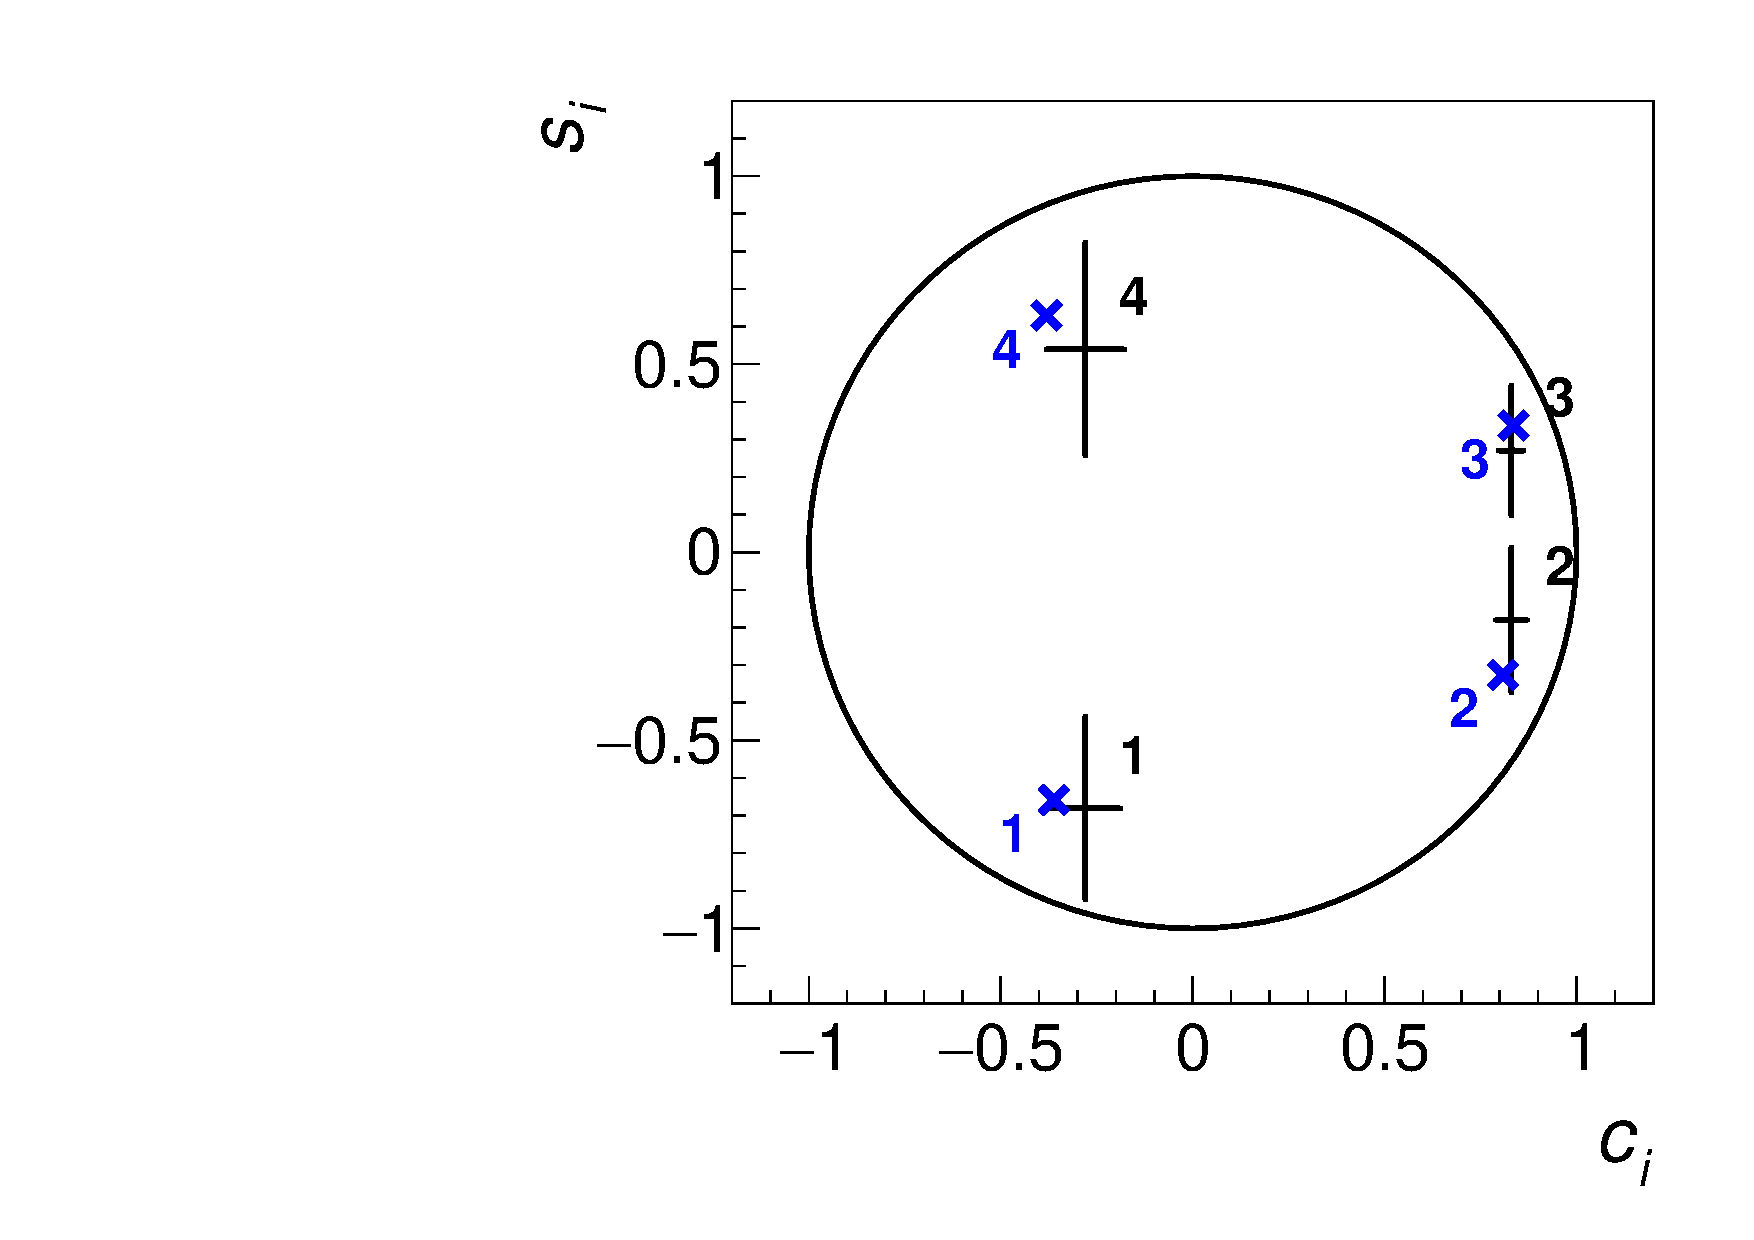
\includegraphics[width=0.9\textwidth]{Plots/cisi_FitResults_Model.pdf}
      \end{figure}
    \end{column}
  \end{columns}
  \begin{center}
    Measured values (black) are consistent and close to LHCb model predictions (blue), so central value of $\gamma$ is not expected to change much
  \end{center}
\end{frame}

\begin{frame}{BESIII preliminary $D^0\to\pi^+\pi^-\pi^+\pi^-$ strong-phase results}
  \vspace{0.3cm}
  \begin{itemize}
    \setlength\itemsep{1.0em}
    \item{Binned strong-phase analysis of $D^0\to\pi^+\pi^-\pi^+\pi^-$ uses the $2\times5$ ``optimal'' binning scheme with $3$~fb$^{-1}$ $\psi(3770)$}
    \item{Earlier CLEO-c analysis with $0.8$~fb$^{-1}$ \href{https://link.springer.com/article/10.1007/JHEP01(2018)144}{JHEP \textbf{01} (2018) 144}}
    \item{New BESIII analysis uses a new binning scheme optimised with a BESIII amplitude model \href{https://arxiv.org/abs/2312.02524}{arXiv:2312.02524}}
    \begin{itemize}
      \item{Amplitude model constructed from a larger data set}
      \item{In principle more sensitive}
    \end{itemize}
    \item{Two binning schemes are available:}
    \begin{itemize}
      \item{We use the more sensitive ``optimal'' binning with $Q = 0.85$}
      \item{The other ``equal $\delta$'' binning has $Q = 0.80$}
    \end{itemize}
    \item{Analysis also approved by review committee, currently in paper review}
  \end{itemize}
\end{frame}

\begin{frame}{BESIII preliminary $D^0\to\pi^+\pi^-\pi^+\pi^-$ strong-phase results}
  \begin{center}
    Small differences between model prediction and measurement, but data points are generally close to the unit circle
  \end{center}
  \vspace{-0.3cm}
  \begin{columns}
    \begin{column}{0.50\textwidth}
      \vspace{-0.5cm}
      \begin{align*}
        c_1 =& +0.12 \pm 0.09 \pm 0.02 \\
        s_1 =& -0.42 \pm 0.21 \pm 0.04 \\
        c_2 =& +0.74 \pm 0.04 \pm 0.02 \\
        s_2 =& -0.39 \pm 0.16 \pm 0.06 \\
        s_3 =& -0.25 \pm 0.12 \pm 0.03 \\
        c_3 =& +0.81 \pm 0.03 \pm 0.01 \\
        c_4 =& +0.42 \pm 0.06 \pm 0.02 \\
        s_4 =& +0.86 \pm 0.19 \pm 0.07 \\
        c_5 =& -0.27 \pm 0.09 \pm 0.03 \\
        s_5 =& -0.22 \pm 0.25 \pm 0.08
      \end{align*}
    \end{column}
    \begin{column}{0.50\textwidth}
      \begin{figure}
        \centering
        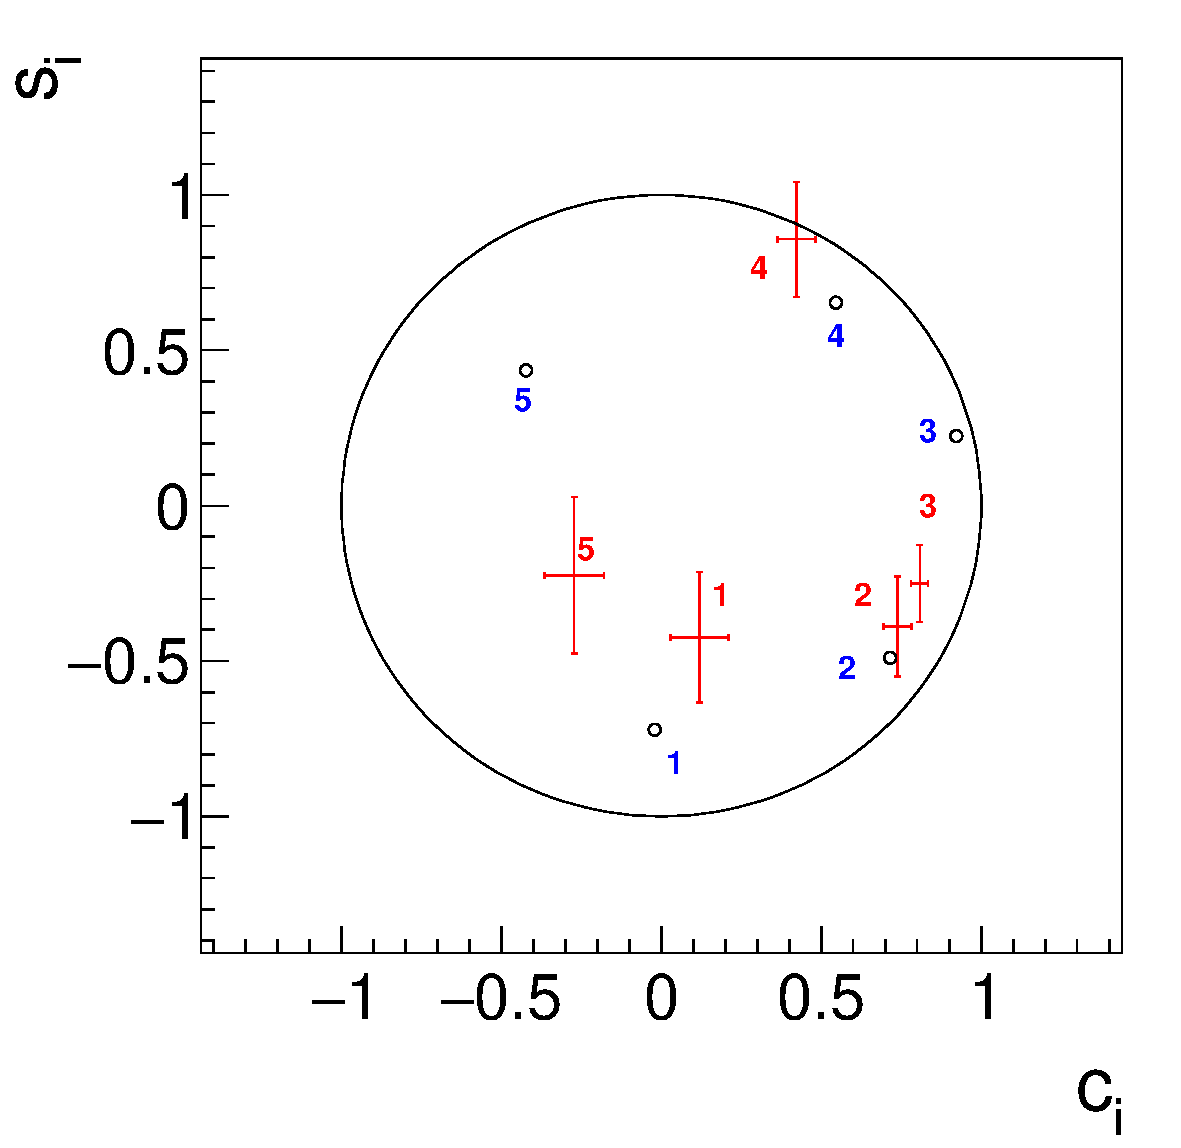
\includegraphics[width=1.0\textwidth]{Plots/CiSiOptim.pdf}
      \end{figure}
    \end{column}
  \end{columns}
  \begin{center}
    Plan: Publish measurement of $\gamma$ using both $K^+K^-\pi^+\pi^-$ and $\pi^+\pi^-\pi^+\pi^-$
  \end{center}
\end{frame}

\section{Summary and next steps}

\begin{frame}{Summary and next steps}
  \vspace{0.0cm}
  {\Large In summary:}
  \vspace{0.5cm}
  \begin{enumerate}
    \setlength\itemsep{1.0em}
    \item{BESIII results approved, paper in review}
    \item{Model-independent measurement of $\gamma$ with $B^\pm\to[h^+h^-\pi^+\pi^-]_Dh^\pm$ presented to B2OC, and ANA note circulated to B2OC conveners}
    \item{$3\sigma$ tension in $D\to K^+K^-\pi^+\pi^-$ has reduced to less than $2\sigma$ due to:}
    \begin{enumerate}
      \item{Non-Gaussian uncertainties in $y_\pm^{DK}$ originating from $s_i$ uncertainties}
      \item{Large anti-correlation between $\gamma$ and $\delta_B^{DK}$}
    \end{enumerate}
    \item{Main takeaway: Important to meausure $\gamma$ \underline{model independently}!}
  \end{enumerate}
\end{frame}

\begin{frame}{Summary and next steps}
  \vspace{0.0cm}
  {\Large Next steps:}
  \vspace{0.5cm}
  \begin{itemize}
    \setlength\itemsep{1.0em}
    \item{Aim to finish thesis by the end of June}
    \item{Unfortunately I failed to obtain useful TORCH results...}
    \item{...but it was a useful experience with testbeam and RICH work!}
    \item{Future plans: Start new postdoc position in Heidelberg in September}
  \end{itemize}
  \vspace{0.4cm}
  \begin{center}
    {\huge Thanks for your attention and thanks for all your support during my PhD!}
  \end{center}
\end{frame}

\end{document}